\section{溶液濃度の影響}

先ほどの節では,密度による落下球高速化への影響を議論したが,本節では溶液濃度による高速化への影響に関して考える.

PAA溶液濃度と終端速度の関係をFig.\ref{fig:concentrationUT}に示す.溶液濃度が濃くなると,終端速度が遅くなることが分かった.PAA溶液濃度と高速化度合の関係をFig.\ref{fig:concentrationUdiff}に示す.縦軸は高速化度合$U_\text{on}/U_\text{off}$,横軸はPAA溶液濃度である.アルミニウム,アルミナにおいてはPAA濃度1wt.\%をピークとして高速化が見られた.一方でステンレスは明瞭な高速化のピークが見られなかったが,PAA濃度0.7-1.3wt.\%のいずれかに高速化のピークが存在すると考えられる.また,真鍮においてPAA濃度0.7wt.\%をピークとして高速化が見られた.これらより,濃度が濃くなると高速化が顕著になるが,濃すぎると高速化がみられにくくなることが分かった.

式(\ref{eq:UdiffRho})を用いて,落下球の密度,溶液濃度の影響を整理した結果をFig.\ref{fig:concentrationUdiffAll}に示す.先述のFig.\ref{fig:rhoUdiffAll}よりも弱い正の相関がみられた.落下球の高速化に対して,粘性による影響よりも密度による影響がより大きいと分かった.

\begin{figure}[ht]
    \centering
    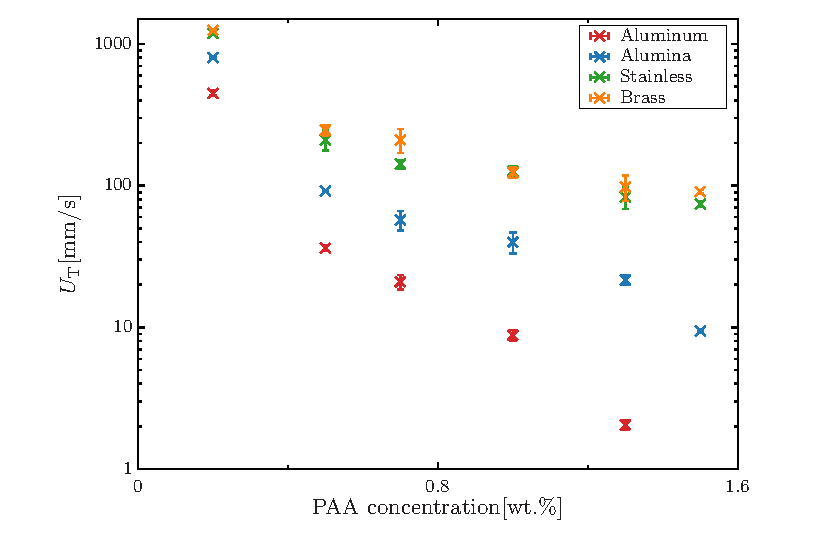
\includegraphics[width=0.8\textwidth]{./5-Results/concentrationUT.eps}
    \caption{Termination velocity in PAA solution concentration.}
    \label{fig:concentrationUT}
\end{figure}

\begin{figure}[ht]
    \centering
    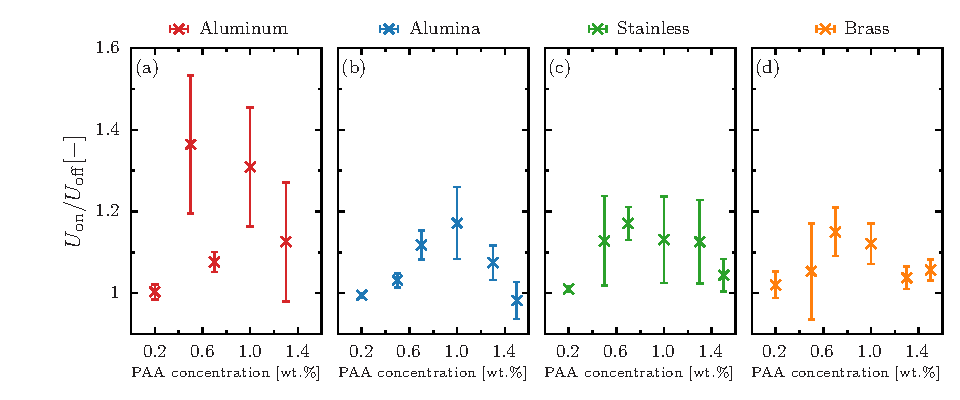
\includegraphics[width=1.0\textwidth]{./5-Results/concentrationUdiff.eps}
    \caption{Velocity ratio in PAA solution concentration (a)Aluminum, (b)Alumina, (c)Stainless, (d)Brass.}
    \label{fig:concentrationUdiff}
\end{figure}

\begin{figure}[ht]
    \centering
    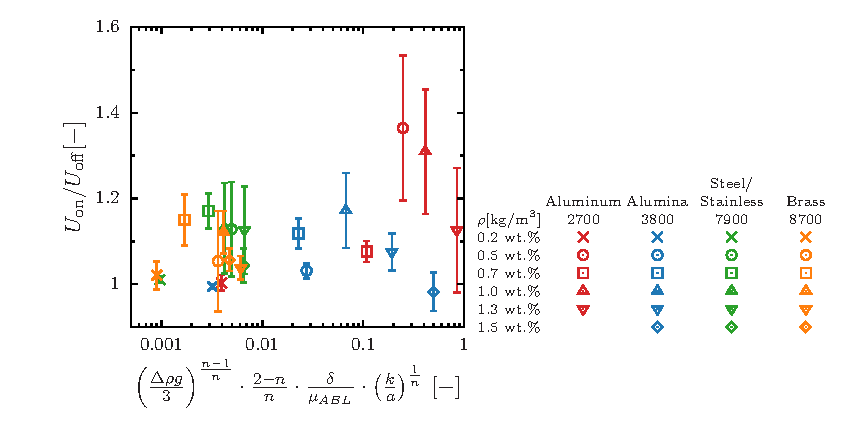
\includegraphics[width=1.0\textwidth]{./5-Results/concentrationUdiffAll.eps}
    \caption{Relationship between density, viscosity and terminal velocity.}
    \label{fig:concentrationUdiffAll}
\end{figure}